\section{Motivation}
\label{sec:motivation}

\asplostodo{This section intentionally preserves the MICRO motivation and its GEMV/KNN figures. Before submission, rerun the general-purpose LLM study under the final ASPLOS protocol. Add a structured-action baseline receiving the same action sites/domains and objective/device/budget/clock context as \framework; report schema, compile/simulation, synthesis, and resource-feasibility rates separately. Keep the existing figure if the rerun supports the same qualitative message; otherwise update its points/caption rather than redesigning the section.}
\subsection{Structural nature of HLS optimization}
\label{subsec:hls-structural}

\iffalse

\begin{itemize}
    \item Domikh sysxetish metaksy pragmas 
    \item paradeigma me array partitioning me factor 2 kai unroll full.
\end{itemize}

\fi
HLS optimization is inherently structural, as performance depends not only on selecting and placing directives, but also on their interactions, which collectively shape the generated hardware. Directives influence key aspects such as parallelism and memory access, and are tightly interdependent. For example, array partitioning determines available memory bandwidth, which constrains achievable parallelism through loop unrolling. In Listing~\ref{alg:gemv-hls}, partitioning arrays \textit{A} and \textit{x} with a factor of $2$ makes an inner loop unroll factor of $8$ infeasible, as the memory system cannot supply operands fast enough to sustain parallel execution. Such imbalances lead to resource underutilization and degraded performance. Consequently, HLS optimization requires reasoning over a tightly coupled design space, where QoR is determined by the global hardware organization rather than isolated directive choices, motivating models that capture structural dependencies and their interactions.

% HLS optimization is inherently structural, as performance improvements arise not only from selecting appropriate directives and placing them correctly, but also from identifying effective combinations that collectively reshape the underlying hardware architecture. 
% HLS directives influence key architectural aspects such as parallelism and memory access patterns, thereby directly impacting the efficiency of the generated design.
% These transformations are highly interdependent, and the impact of one directive depends on the configuration of others. 
% For example, array partitioning determines the available memory bandwidth, which in turn constrains the achievable parallelism through loop unrolling. 
% In the running example of Listing~\ref{alg:gemv-hls}, if arrays \textit{A} and \textit{x} are partitioned with a factor of $2$, applying an inner loop unroll factor of $8$ becomes infeasible, since the memory system cannot provide the required operands simultaneously to sustain parallel execution. 
% Such imbalances between compute parallelism and memory bandwidth lead to under-utilization of hardware resources and degraded performance.
% Consequently, HLS optimization requires reasoning over a tightly coupled design space, where QoR is determined by the global organization of the hardware rather than isolated directive choices, motivating the need for models that can capture structural dependencies and their interactions across the program.

\subsection{Limitations of Decoder-Only LLMs for HLS}
\label{subsec:llm-limitations}

\iffalse

\begin{itemize}
    \item Motivate the inefficiency of current models (ChatGPT, Claude, Deepseek, LLaMa) to provide efficient pragmas. Evaluate the models on:
    \begin{itemize}
        \item Structural legality
        \item PPA improvement
        \item Resource feasibility
    \end{itemize}

    \item Categorize failure modes:
    \begin{itemize}
        \item Dependency violations (illegal pipelining)
        \item Memory port conflicts
        \item Misplaced pragmas
        \item Over-aggressive unrolling
    \end{itemize}
    \item \textbf{Syntax vs. Structural correctness.} We can show that:
    \begin{itemize}
        \item Syntax correctness (e.g., the pragmas are placed correctly in the right positions) is high
        \item Structural correctness (e.g., inter-pragma dependencies and resource constraints) is significantly lower
    \end{itemize}

    \item \textbf{Kernel sensitivity assessment:} Ideally we can show that for less complex kernels they work well (Loop depth, Memory intensity, Graph size), but for more complex they fail.
    \item Small Pareto teaser for these two kernels Fig.~\ref{fig:llm-decoder-limitation}
\end{itemize}

\fi


\begin{figure}[t]
    \centering
    
\includegraphics[width=\linewidth]{figures/03__Motivation/LEGEND-GEMV-KNN-crop.pdf}
    \\
\begin{subfigure}[b]{0.48\linewidth}  % First subfigure
        \centering
        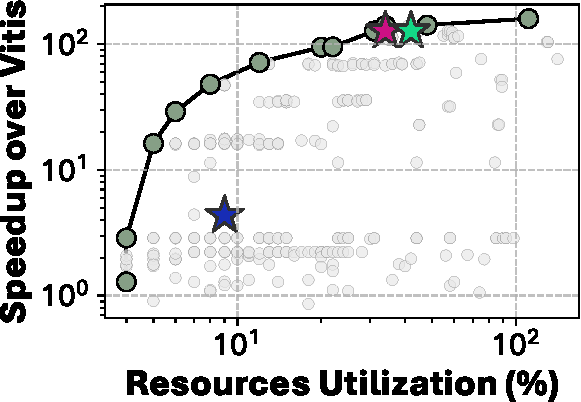
\includegraphics[width=\linewidth]{figures/03__Motivation/GEMV_PF-crop.pdf}
        \caption{GEMV}
        \label{fig:gemv-pf}
    \end{subfigure}
    \hfill
    \begin{subfigure}[b]{0.48\linewidth}  % Second subfigure
        \centering
        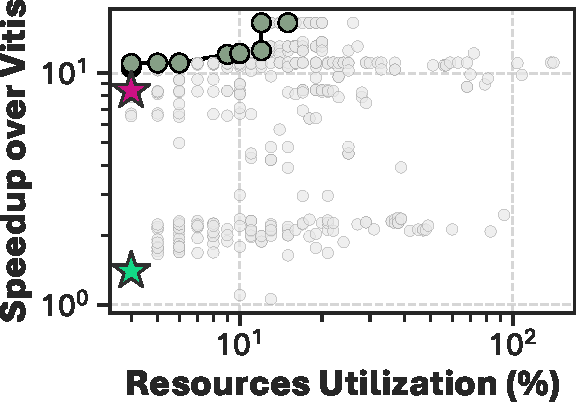
\includegraphics[width=\linewidth]{figures/03__Motivation/KNN_PF-crop.pdf}
        \caption{KNN}
        \label{fig:knn-pf}
    \end{subfigure}
% optional spacing between figures and legend
    \caption{Positioning of decoder-only LLM generated designs compared to Pareto-optimal configurations from ~\cite{ferikoglou2026gnomegasis}.}
    \label{fig:llm-decoder-limitation}
\end{figure}

Modern large-scale LLMs, such as GPT-4o~\cite{openai2023gpt4} and Claude Haiku 4.5~\cite{anthropic2024claude3}, follow a decoder-only architecture, modeling code as a sequence of tokens and capturing semantic relationships through autoregressive attention. 
While this enables strong capabilities in code understanding and generation~\cite{chang2024survey}, it inherently limits their ability to explicitly model structural dependencies in programs.
However, as discussed in \S\ref{subsec:hls-structural}, in HLS performance optimization is fundamentally driven by structural transformations and their interactions. 
Although LLMs benefit from strong generalization and extensive training on large code corpora, their token-centric reasoning often fails to capture hardware-level constraints and dependencies required for effective directive optimization.

% Decoder-only LLMs, such as GPT-4o and Claude Haiku 4.5, have gained widespread adoption due to their strong ability to understand and generate semantically coherent text~\cite{chang2024survey}.
% However, these models operate by capturing semantic patterns and token-level dependencies, often failing to account for the structural properties that are intrinsic to many specialized domains.

% In the context of HLS, this shortcoming becomes particularly evident.
% As discussed earlier, performance optimization in HLS is fundamentally driven by structural transformations rather than purely semantic reasoning~\cite{masouros2024late, bai2023towards}.
% Consequently, approaches that rely primarily on semantic pattern recognition may struggle to effectively explore and exploit the HLS design space.
To systematically investigate these limitations, we evaluate the capability of decoder-only LLMs to optimize HLS designs through prompt-based interaction. 
We consider three applications of increasing complexity: (i) the GEMV kernel of Listing~\ref{alg:gemv-hls}, (ii) a K-Nearest Neighbors (KNN) implementation from the RodiniaHLS benchmark suite~\cite{cong2018understanding}, and (iii) a Kalman filtering application sourced from GitHub.
The LLMs are instructed to minimize latency under resource constraints on an AMD UltraScale+ ZCU104 platform (100 MHz), restricted to pragma insertion without modifying the source code.
We evaluate GPT-4o, Claude Haiku 2.5, and Gemini 2.5 Pro. Generated designs are synthesized with Vitis HLS 2021.1 and assessed in terms of latency speedup and resource utilization against a baseline without directives (Vitis). To contextualize performance, we derive Pareto-optimal configurations using an NSGA-II-based design space exploration framework~\cite{ferikoglou2026gnomegasis}.
% In all cases, the optimization objective is to minimize latency through the insertion of HLS directives, while adhering to the resource constraints of an AMD UltraScale+ ZCU104 platform operating at 100 MHz. 
% Importantly, the LLMs are restricted to introducing HLS pragmas only, without modifying the original source code, thereby isolating their ability to reason about structural optimizations.
% We evaluate the performance of three widely used LLMs, namely GPT-4o, Claude Haiku 2.5, and Gemini 2.5 Pro.
% Each generated design is synthesized using Vitis HLS 2021.1 and assessed in terms of latency speedup relative to a baseline implementation without HLS directives (referred to as Vitis), as well as resource utilization.
% Additionally, we compare against the default compiler-driven optimization level (Vitis -O3) to establish a strong automated baseline.
% Finally, to contextualize the quality of the LLM-generated solutions, we perform a system-level design space exploration using an NSGA-II-based optimization framework~\cite{ferikoglou2026gnomegasis}. 
% This allows us to derive the Pareto frontier for the target FPGA and clock frequency, providing a reference for how closely the LLM-derived designs approach optimal trade-offs between latency and resource usage.

Figure~\ref{fig:llm-decoder-limitation} shows the Pareto frontiers obtained via NSGA-II and the LLM-generated designs for GEMV and KNN.
% Figure~\ref{fig:llm-decoder-limitation} illustrates the Pareto frontiers obtained from the NSGA-II–based exploration framework, alongside the designs generated by the evaluated LLMs for the GEMV and KNN applications.
For GEMV, the latency-efficient Pareto design achieves a $159.5\times$ speedup over baseline Vitis, using 1\%, 11\%, 34\%, and 65\% of BRAM, DSP, FF, and LUT, respectively. 
In contrast, Gemini 2.5 Pro attains only $4.4\times$, failing to identify the \textit{y} array as critical for throughput. 
As a result, no partitioning is applied, creating a memory bottleneck that prevents achieving an initiation interval (II) of 1 and limits the benefits of loop unrolling.
In contrast, GPT-4o and Claude Haiku 2.5 correctly identify \textit{y} as performance-critical and apply appropriate partitioning, enabling efficient memory access and sustained pipeline throughput, achieving up to $127.2\times$ speedup within resource constraints.
% Focusing on GEMV, the most Latency-Efficient (LE) design on the Pareto front achieves a speedup of $159.5\times$ over the baseline Vitis implementation, while utilizing 1\%, 11\%, 34\%, and 65\% of BRAM, DSP, FF, and LUT resources, respectively. 
% In contrast, Gemini 2.5 Pro attains only a $4.4\times$ speedup, falling significantly short of the achievable performance. 
% To be more specific, this limitation stems from its failure to recognize the \textit{y} array as critical for sustaining throughput. 
% Consequently, no partitioning directives are applied, leading to an implementation where \textit{y} is mapped to a memory with limited access ports. 
% This creates a structural bottleneck at the write stage, preventing the pipeline from maintaining an Initiation Interval (II) of $1$ and ultimately limiting the benefits of loop unrolling.
% In contrast, both GPT-4o and Claude Haiku 2.5 correctly identify \texttt{y} as a performance-critical array and apply the appropriate directives. 
% This enables efficient memory access, sustains pipeline throughput, and results in a speedup of $127.2\times$, while adhering to the resource constraints of the target FPGA.

Regarding KNN, the latency-efficient Pareto design achieves a $17\times$ speedup over baseline Vitis, while utilizing only 1\%, 1\%, 2\%, and 11\% of BRAM, DSP, FF, and LUT resources, respectively. In contrast, Gemini 2.5 Pro generates directives that result in a compilation failure. 
Specifically, it introduces dataflow without properly restructuring memory accesses, causing multiple processes to read concurrently from the same global memory interface and violating the single-port constraints of bundled AXI interfaces in Vitis HLS.
This behavior highlights a key limitation of general-purpose LLMs, which often fail to account for hardware-level constraints.
A similar issue is observed with Claude Haiku 2.5: although loop unrolling is applied, the corresponding arrays are not partitioned, preventing true parallel memory access and limiting performance to $1.4\times$ speedup. In contrast, GPT-4o adopts a more balanced strategy by combining pipelining (II=1), dataflow, and proper memory management, achieving a higher speedup of $8.4\times$, which nevertheless remains well below the optimal achievable performance.

% Regarding the KNN application, the latency-efficient design on the Pareto front achieves a speedup of $17\times$ over the baseline Vitis implementation, while utilizing only 1\%, 1\%, 2\%, and 11\% of BRAM, DSP, FF, and LUT resources, respectively.
% In contrast, Gemini 2.5 Pro generates directives that result in a compilation failure. 
% Specifically, the model introduces a dataflow optimization without properly restructuring memory accesses, leading to multiple processes attempting to read concurrently from the same global memory interface. 
% This violates the single-port access constraints of bundled AXI interfaces in Vitis HLS, ultimately causing synthesis to fail. 
% \textit{This behavior highlights a key limitation of general-purpose LLMs, which often lack the domain-specific knowledge required to reason about hardware-level constraints and produce valid, high-performance designs}.
% A similar limitation is observed with Claude Haiku 2.5. 
% Although loop unrolling directives are applied, the corresponding arrays are not partitioned, preventing the exploitation of true parallel memory access. 
% As a result, the potential benefits of unrolling are not realized, leading to a modest speedup of only $1.4\times$.
% In contrast, GPT-4o achieves a more balanced and effective optimization strategy. 
% By applying pipelining with an II of $1$, appropriately managing array accesses, and introducing dataflow at the top level, it enables efficient overlap of computation stages. 
% This results in a significantly improved speedup of $8.4\times$, which nevertheless remains well below the optimal achievable performance.

Finally, for the Kalman filter, which is the most complex application considered, the latency-efficient Pareto design achieves a $35.3\times$ speedup over baseline Vitis, with resource utilization of 92\%, 7\%, 7\%, and 19\% for BRAM, DSP, FF, and LUT, respectively.
In this case, GPT-4o generates directives that lead to compilation failure due to misplaced array pragmas, applied before their corresponding declarations, which result in undefined variable errors.
For Claude Haiku 2.5 and Gemini 2.5 Pro, both models apply overly aggressive directives, leading to BRAM over-utilization of up to 113\%. \textit{This behavior highlights the difficulty for general-purpose LLMs to consistently satisfy hardware resource constraints, often leading to impractical designs.}


\subsection{Pitfalls of Structure-Agnostic Adaptation}

\iffalse

\begin{figure}[t]
    \centering
    \includegraphics[]{example-image-duck}
    \caption{Evaluation of text-adapted LLMs}

    \label{fig:llm-decoder-limitation}
\end{figure}


\begin{itemize}
    \item Describe what is structure-agnostic adaptation
    \begin{itemize}
        \item Prompt engineering (goal-specific prompts, detailed instructions)
        \item Retrieval-augmented generation (RAG)
        \item qLoRA
        \item instruction tuning
        \item say that these models Operate entirely in token space, do not introduce explicit structural representations and do not alter the model’s reasoning topology.
    \end{itemize}
    \item Saturation of Text-Based Adaptation. Evaluate:
    \begin{itemize}
        \item Evalute Prompt-engineered variant, 
        \item RAG variant
        \item qLoRA-only variant
        \item We should see that structural error rates remain high across adaptation strategies. 
    \end{itemize}
    \item Explain why this happens
    \begin{itemize}
        \item Prompts encode intent but not invariants.
        \item Retrieval provides examples but not dependency compression.
        \item Fine-tuning optimizes token likelihood, not graph consistency.
        \item Structural constraints are non-local and combinatorial.
    \end{itemize}
\end{itemize}

\fi

High-level adaptation techniques, such as prompt engineering~\cite{pan2025survey} and retrieval-augmented generation (RAG)~\cite{lewis2020retrieval}, aim to guide LLMs through additional context and structured instructions. 
This concept has also been investigated in the HLS domain~\cite{xiong2024hlspilot}, where enriched prompts explicitly specify which directives should be applied and where they should be placed within the code.
While these approaches improve guidance, they remain fundamentally structure-agnostic, relying on token-level context rather than explicit representations of program structure.

To assess their effectiveness, we design prompts that encode key HLS optimization strategies, including pipelining, loop unrolling, and array partitioning~\cite{ferretti2020leveraging}. Beyond directive placement, the prompts also include tuning guidance (e.g., enforcing II=1 or aligning partitioning factors with loop unrolling). We evaluate this approach on KNN and Kalman filtering, representing the more complex applications.
For KNN, enriched prompts improve performance across models. In particular, Gemini 2.5 Pro generates a valid design by correctly applying dataflow under AXI constraints, achieving an $8.4\times$ speedup over baseline. 
GPT-4o and Claude Haiku 4.5 also benefit, reaching $6\times$ and $15.6\times$ speedups, respectively.
However, this improvement does not generalize to more complex cases. In the Kalman filter, GPT-4o still produces invalid code due to incorrect pragma placement, while Claude Haiku 2.5 and Gemini 2.5 Pro exceed BRAM capacity (up to 113\%), despite explicit guidance.

These results show that, \textit{even with detailed and structured prompts, general-purpose LLMs struggle to consistently generate valid and efficient HLS designs}. While prompt engineering can guide the model toward better local decisions, it does not provide an explicit representation of program structure or hardware constraints. As a result, the model must infer complex structural relationships implicitly from token sequences, which is often unreliable, especially for long-range dependencies and tightly coupled optimizations. This limitation becomes more pronounced as application complexity increases, where multiple interacting transformations must be coordinated. Consequently, structure-agnostic adaptation remains insufficient for reliably navigating the HLS design space.
% Prompt engineering~\cite{pan2025survey} has emerged as an effective strategy for guiding LLMs by providing additional context and structured instructions, with the goal of steering them toward more optimal solutions. 
% This concept has also been investigated in the HLS domain~\cite{xiong2024hlspilot}, where enriched prompts explicitly specify which directives should be applied and where they should be placed within the code.
% In this section, we aim to quantify the extent to which such an approach can improve the quality of the generated designs. 
% We focus on key optimization techniques, including loop pipelining, loop unrolling, array partitioning etc, as these are central to achieving high performance in HLS implementations~\cite{ferretti2020leveraging}.
% Beyond simply indicating directive placement, the prompts also incorporate guidance on how to tune these optimizations. 
% For instance, the model is encouraged to pipeline loops with an II of $1$ and to select array partitioning factors that are consistent with the corresponding loop unrolling factors.
% To evaluate the effectiveness of this strategy, we focus on KNN and Kalman filtering, as they represent the most complex applications among those considered.
% This enables us to assess whether carefully designed prompts can enhance performance and overcome the limitations of decoder-only LLMs in capturing the structural requirements of HLS optimization, while better aligning their outputs with hardware constraints.

% For the KNN application, we observe a clear benefit from providing more structured instructions. 
% When using the enriched prompt with Gemini 2.5 Pro, the additional guidance on applying the dataflow directive enables the model to respect the single-port access constraints of the bundled AXI interface, resulting in a design that achieves a speedup of $8.4\times$ over the Vitis baseline. 
% More generally, the improved and more precise directive guidance enhances the performance of the other models as well, with GPT-4o achieving a $6\times$ speedup compared to the simpler prompt and Claude Haiku 4.5 showing a significant improvement, reaching $15.6\times$.
% However, this trend does not extend to the Kalman filter application. 
% Despite explicitly specifying directive placement, GPT-4o still generates incorrect code by placing array partition directives before the corresponding array declarations, leading to compilation errors. 
% Similarly, although the enriched prompt includes guidance on resource-aware optimizations, both Claude Haiku 2.5 and Gemini 2.5 Pro produce designs that exceed the available BRAM capacity, reaching 113\% utilization.
% These observations indicate that, \textit{even with detailed and structured guidance, general-purpose LLMs struggle to consistently generate valid and efficient HLS designs}, highlighting inherent limitations in their ability to capture and enforce hardware-specific constraints.


\paragraph{ASPLOS extension: target constraints beyond prompt-only guidance.}
The MICRO motivating study focused primarily on whether general-purpose LLMs could coordinate structural HLS optimizations from text. The revised evaluation additionally separates this question from target conditioning. All applicable baselines receive the same optimization objective and explicit device/resource/clock request, and the task-specific Stage~1 model provides the direct control for the benefit of supervised domain adaptation. This distinction is important because the final framework should attribute gains to the proposed structural fusion only after accounting for both prompt engineering and HLS-specific fine-tuning.

\asplostodo{If space is tight, retain only one detailed directive trace (preferably KNN or Kalman) and move the remaining per-model anecdotes to the appendix. Use the main-body space for the aggregate validity/feasibility and objective-regret result requested by MICRO reviewers.}

\iffalse

\subsection{Different Optimization Goals}

\begin{itemize}
    \item This is to motivate the need for different adapters.
\end{itemize}

\fi